\documentclass[11pt,a4paper]{article}
\usepackage {amsmath, amssymb, amsfonts}
\usepackage {graphics}
\usepackage {graphicx}
\usepackage{placeins}

\usepackage{hyperref}
\usepackage{float}
\usepackage{csquotes}
\usepackage[linesnumbered, ruled,longend]{algorithm2e}
\usepackage{amsmath}
\usepackage{bbm}
\usepackage[scaled]{helvet}
\usepackage[cm]{sfmath}
\usepackage[T1]{fontenc}
\renewcommand{\familydefault}{\sfdefault}
\usepackage[doublespacing]{setspace}
\usepackage{sansmath}
 %\usepackage{algorithmicx,algpseudocode}
\usepackage{anysize}
\usepackage{siunitx}
\usepackage{mathtools}
\usepackage{multicol}
\usepackage{todonotes}

\usepackage{xcolor}

%\usepackage{lineno}
%\linenumbers

\topmargin 0.0cm
\oddsidemargin 0.2cm
\textwidth 16cm 
\textheight 23cm
\footskip 1.0cm

\renewcommand\Re{\operatorname{Re}}
\renewcommand\Im{\operatorname{Im}}
\DeclareMathOperator{\argmax}{argmax}
\DeclareMathOperator{\argmin}{argmin}

\newtheorem{lemma}{Lemma}
\newtheorem{theorem}{Theorem}
\newtheorem{proposition}{Proposition}
\newtheorem{remark}{Remark}
\newtheorem{corollary}{Corollary}

\usepackage{color,soul}
\newcommand{\nonl}{\renewcommand{\nl}{\let\nl\oldnl}}% Remove line number for one line
\newcommand{\mymathsf}[1]{\mbox{\sansmath$\mathsf{#1}$}}
\SetKw{KwGoTo}{go to}

\usepackage[backend=bibtex, style=numeric, sorting=none]{biblatex} 
\addbibresource{BK_chaos} 

\begin{document}
\title{Machine-learning informed gapfilling}
\author{Behzad D. Karkaria$^{1}$ Kiran R. Patil$^{1}$\\
\normalsize{$^{1}$MRC Tox}\\
\\
\normalsize{$^\ast$To whom correspondence should be addressed;}\\
\normalsize{E-mail: }
}
\date{}

\maketitle
\begin{abstract}
    Genome scale metabolic model reconstructions are relatively poor at predicting species viability in specified media. Methods such as gap-filling, require experimental data to identify which metabolic reactions should be added to achieve species growth. However, this therefore requires \textit{in vitro} screening of each species in different media environments. We have developed a machine learning pipeline that can predict the viability of a microbial species in a given defined media. We propose that this pipeline can be used to perform automatic gap-filling, to improve the output of existing automated metabolic reconstruction frameworks.
\end{abstract}

\section{Introduction}
Genome-scale metabolic models (GSMMs) are mathematical representations of an organisms metabolism. GSMMs are automatically reconstructed, using tools such as CarveMe an gapseq. These tools use associatons between genomes and gene annotation databases to construct a biochemical network, represented as a stoichiometry matrix. However, these models require curation informed by organism-media viability experiments. If an organism is viable in a defined media, the model has may need reactions added to ensure the model yields the same phenotype as the experiment.
\section{Results}
GSMM reconstruction is...
Our dataset is composed of 92 species of gut bacteria, grown in 10 different media (Figure~\ref{fig:FIG_dataset}.) Figure~\ref{fig:FIG_dataset}a shows the media compositions. All media use glucose as a carbon source. All strains were inoculated at 0.01 OD, if the OD after 48hrs of culture was less than 0.1, we defined this strain as inviable in the media. Figure~\ref{fig:FIG_dataset}b shows the viability of each species in each media.
\\\\
\hl{Describe dataset}
\begin{figure}[tbp]
    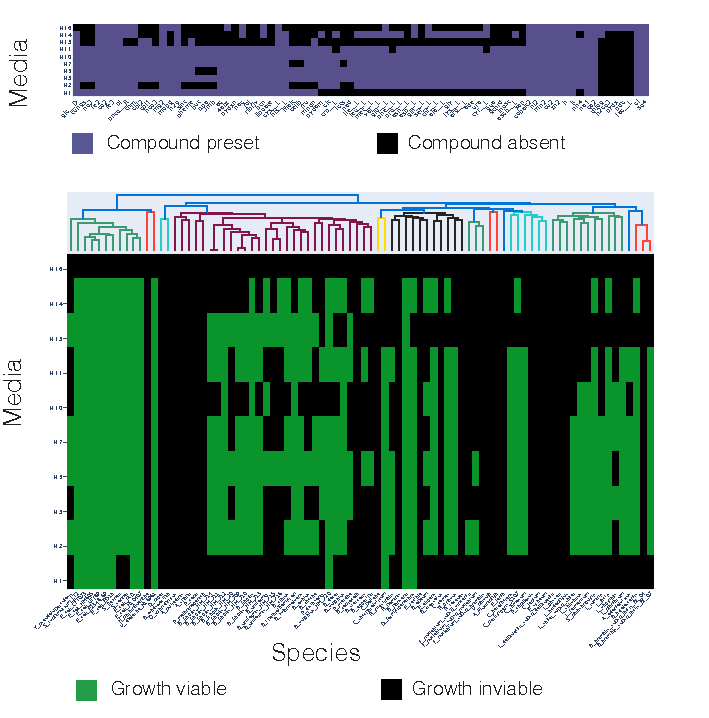
\includegraphics[width=\textwidth]{figures/FIG_dataset/FIG_dataset.pdf}
    \caption{}
    \label{fig:FIG_dataset}
 \end{figure}

\subsection*{Raw GSMMs are poor predictors of growth}
Automated GSMM reconstruction are poor predictiors of growth. To illustrate this, we reconstructed all 92 models for species shown in Figure~\ref{fig:FIG_dataset}B. We refer to these uncurated, automatically constructed GSMMs as raw GSMMs. For each raw GSMM-media combination, we set the media concentrations and optimize to find the growth rate ($\mu$). Where $\mu > 0$ we classifiy viabile growth, where $\mu < 0$ we classifiy inviabile growth. The performance of these raw GSMMs on the dataset are shown in Figure~\ref{fig:FIG_raw_GSMM_performance}a. The confusion matrix shown in and performance metrics show that these raw GSMMs suffer from frequent false negatives (Figure~\ref{fig:FIG_raw_GSMM_performance}b). This can be due to poor assembly quality and incomplete genome annotation datasets. 
\begin{figure}[tbp]
    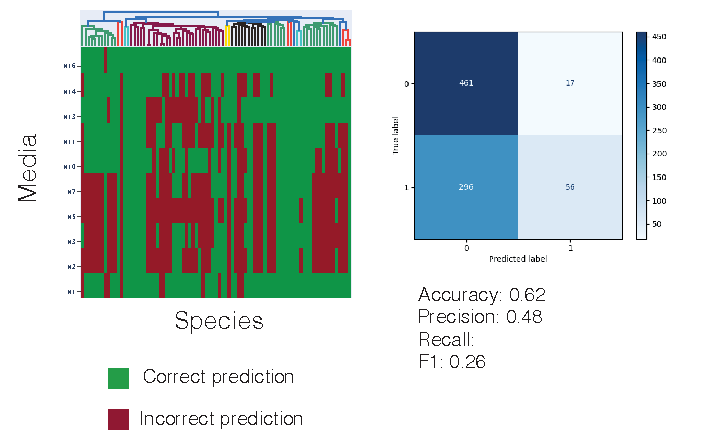
\includegraphics[width=\textwidth]{figures/FIG_mel_raw_GSMM_classifier/FIG_raw_GSMM_performance.pdf}
    \caption{Performance of raw GSMMs as classifiers of growth}
    \label{fig:FIG_raw_GSMM_performance}
 \end{figure}

\subsection*{Integrating metabolism and media for viability classification}
While the raw GSMMs are poor predictors of growth, we hypothesised that features of the raw GSMMs, paried with features of the defined media could be leveraged by machine learning techniques to predict species-media vialility.
\\\\
As illustrted by Figure~\ref{fig:FIG_raw_GSMM_performance}, raw GSMMs are incomplete and possibly incorrect representations of an organism. However, we expected this fuzzy representation to useful for predicting media-species viability. Here we demonstrate machine learning approaches that integrate information about the organism metabolism and the media environment to classify strain viability.
\\\\
We reprsent each organism as a binary set of features indicating presence or absenece of a metabolic reaction in the raw GSMM ($X_{Model}$). We refer to this as a metabolic fingerprint. Similarly, each defined media is represented as a binary presence or absesnce of a compound ($X_{Media}$). Binary lables indicate growth for each media-species combination ($y_{g}$), as shown in Figure~\ref{fig:FIG_dataset}. 
\\\\
First, we generate a test set consisting of 20\% of the whole dataset. The strains reserved for the test set were selected by traversing the x-axis shown in Figure~\ref{fig:FIG_raw_GSMM_performance}, and selecting every \hl{n}th strain. Validation sets were generated by randomly sampling from 20\% of the training data (\hl{x strains}). The training set therefore consists of \hl{x strains}.
\\\\
We decided to compare Random Forest, Gradient Boosting, support vector machines (SVM) and decision trees. We performed a gridsearch hyperparameter optimisation for each model. For each set of parameters, fitting was repeated 10-times to account for the stochastic behaviour of the models and the variation in sampling of the validation set. Optimal hyperparameters were chosen by the highest mean validation F1-score. We focus on the F1-score because we are more interested in correcly classifying strain viability than correctly classifying inviable strains. Figure~\ref{fig:FIG_model_selection} shows a comparison optimised models. We can see that random forest, gradient boosting and SVM classifiers all perform similarly. Table~\ref{tab:TAB_model_performance} shows the mean and standard deviations of each optimised model. Furthermore, we can see that the trained classifiers performance on the validation set greatly exceeds the performance of raw GSMMs on the entire dataset. 
\begin{figure}[tbp]
    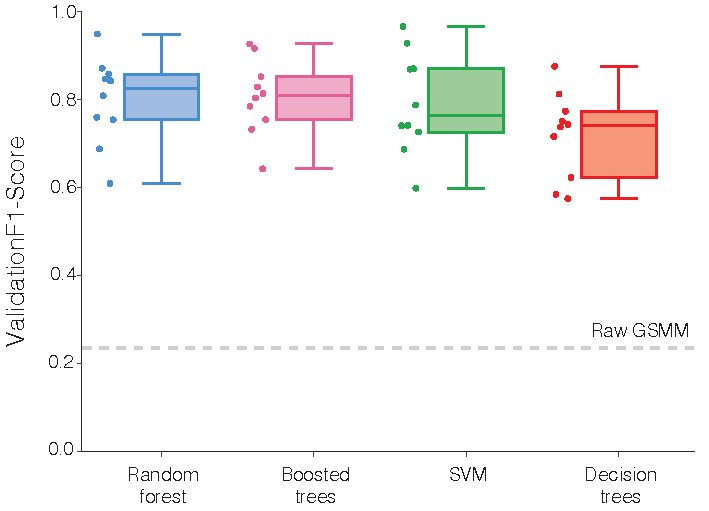
\includegraphics[width=\textwidth]{figures/FIG_model_selection/FIG_model_selection.pdf}
    \caption{Comparison of trained classifier validation F1-scores}
    \label{fig:FIG_model_selection}
\end{figure}

\begin{center}
    \begin{tabular}{ | l | l | l | l | l | p{5cm} |}
    \hline
    \textbf{Model} & \textbf{Mean Accuracy} & \textbf{Mean F1-Score} \\ \hline \hline
    Random Forest & 0.82 & 0.80 \\ \hline
    xGBoost & 0.82 & 0.80 \\ \hline
    SVM & 0.81 & 0.79 \\ \hline
    Decision tree & 0.76 & 0.72 \\ \hline
    Raw GSMM & 0.62 & 0.23 \\ \hline
    \end{tabular}
    \label{tab:TAB_model_performance}
\end{center}

Using the optimal hyperparameters identified for random forest (see Methods), we retrained a model using the entire training set, and assessed its performance on the test set. In Figure~\ref{fig:FIG_test_set}A we can see that the classifier performs poorly on \textit{B. animalis subsp lactis BL 04}, \textit{C. bolteae} and \textit{E. eligens}. However, this classifier is a considerable improvement on the performance of raw GSMMs.  
\begin{figure}[tbp]
    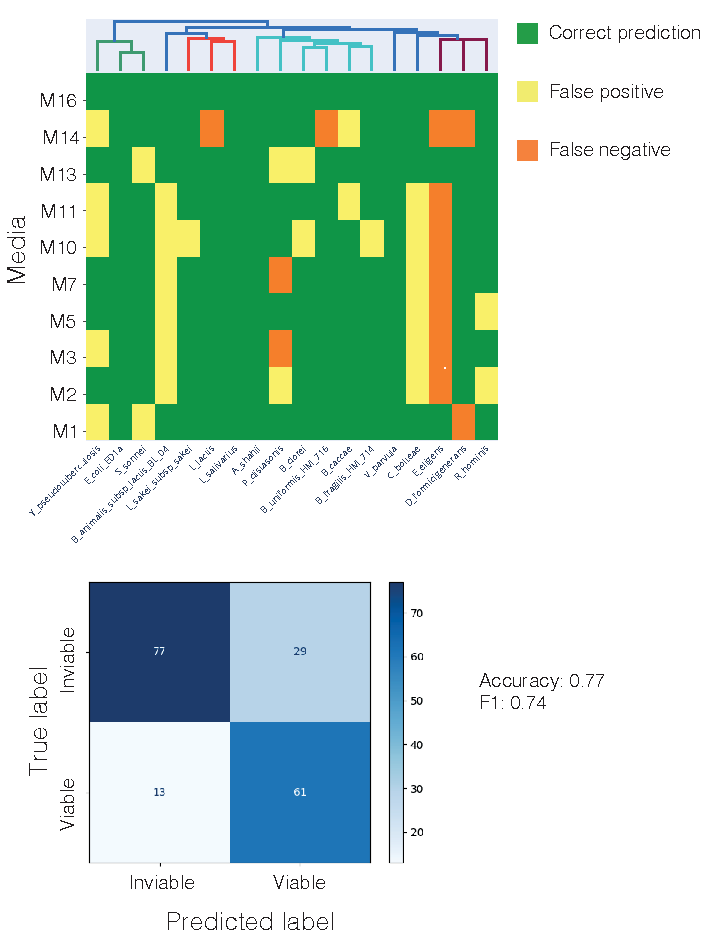
\includegraphics[width=\textwidth]{figures/FIG_test_set/FIG_test_set.pdf}
    \caption{Performance of optimal random forest model on test set.}
    \label{fig:FIG_test_set}
\end{figure}

\subsection*{Automated gapfilling using random forest classifier}
Having trained the classifier on a set of gut bacteria and demonstrated good performance on the test set, we wanted to see if this method was able to provide contextual information about the organism to inform gapfilling.
\\\\
The KOMODO dataset contains information about organism-media pairings to grow difficult-to-culture microbes. We took a subset of this dataset for anaerobes that grow in a range of 6.0 - 7.5pH, loosely matching the data used to train the random forest classifier. This 94 datapoints, consisting of 49 different medias and 93 different organisms. 
\\\\
We reconstructed raw GSMMs of all organisms using CarveMe. We simulated the growth in the growth media defined by the KOMODO dataset. These are media that are known to be culture each organism. The raw GSMMs had a accuracy of zero, always predicting no growth.
\\\\
For each organism, we used the trained random forest classifier to predict if the organism should grown on each of the 10 media used in training. If the classifier predicted growth, we performed gapfilling on the raw GSMM for that media. We then retested resulting 'polished' GSMMs that had been gapfilled as informed by our random forest classifier. 
\\\\
Figure~\ref{fig:FIG_komodo_gapfill} shows the performance of the gapfilled models on the KOMODO dataset. We can see that the performance of these models is still poor, however, we see that 7 polished models now correctly predict growth which the raw GSMMs did not. We believe this is a strong indication that our methods can provide improvements without the need for additional experiments. However, to unlock the true potential of these techinques, we require a larger and more diverse dataset of negative and positive culture data.

\begin{figure}[tbp]
    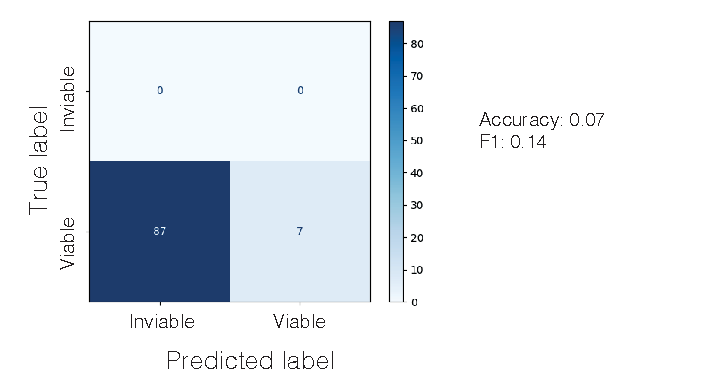
\includegraphics[width=\textwidth]{figures/FIG_komodo_gapfill/FIG_komodo_gapfill.pdf}
    \caption{Performance of KOMODO models following machine learning informed gapfilling}
    \label{fig:FIG_komodo_gapfill}
\end{figure}


\section{Methods}
\subsection*{Model selection hyperparameters}
Models were optimized using a grid search across hyperparameters shown in Table~\ref{tab:TAB_hyperparameters}. All parameters refer to those used in the scikit-learn package. The red highlighted parameters are those which produced the optimal performance for each model.
\begin{table}[]
    \centering
    \begin{tabular}{ll}
    \hline
    \multicolumn{2}{||c||}{\textbf{Random Forest}} \\ \hline
    \multicolumn{1}{|l|}{n estimators} & \multicolumn{1}{l|}{50, \textcolor{red}{250}, 500, 750} \\ \hline
    \multicolumn{1}{|l|}{max depth}    & \multicolumn{1}{l|}{\textcolor{red}{null}, 10}   \\ \hline
    \multicolumn{1}{|l|}{max features}    & \multicolumn{1}{l|}{\textcolor{red}{sqrt}, log2}   \\ \hline
    \multicolumn{2}{||c||}{\textbf{Boosted trees}} \\ \hline
    \multicolumn{1}{|l|}{n estimators} & \multicolumn{1}{l|}{50, \textcolor{red}{250}, 500, 750} \\ \hline
    \multicolumn{1}{|l|}{learning rate} & \multicolumn{1}{l|}{0.1, \textcolor{red}{0.01}, 0.05} \\ \hline
    \multicolumn{1}{|l|}{subsample} & \multicolumn{1}{l|}{1.0, \textcolor{red}{0.5}, 0.75} \\ \hline
    \multicolumn{1}{|l|}{max depth}    & \multicolumn{1}{l|}{null, \textcolor{red}{10}}   \\ \hline
    \multicolumn{1}{|l|}{max features}    & \multicolumn{1}{l|}{\textcolor{red}{sqrt}, log2}   \\ \hline
    \multicolumn{1}{|l|}{tol}    & \multicolumn{1}{l|}{\textcolor{red}{1e-4}} \\ \hline
    \multicolumn{2}{||c||}{\textbf{SVM}} \\ \hline
    \multicolumn{1}{|l|}{C} & \multicolumn{1}{l|}{0.1, 0.01, 1.0, \textcolor{red}{10.0}} \\ \hline
    \multicolumn{1}{|l|}{kernel} & \multicolumn{1}{l|}{\textcolor{red}{rbf}, linear, poly, sigmoid} \\ \hline
    \multicolumn{1}{|l|}{gamma} & \multicolumn{1}{l|}{\textcolor{red}{scale}, auto} \\ \hline
    \multicolumn{1}{|l|}{degree} & \multicolumn{1}{l|}{\textcolor{red}{3}} \\ \hline
    \multicolumn{1}{|l|}{tol} & \multicolumn{1}{l|}{1e-3, 1e-4, \textcolor{red}{1e-2}} \\ \hline
    \multicolumn{1}{|l|}{shrinking} & \multicolumn{1}{l|}{\textcolor{red}{True}} \\ \hline
    \multicolumn{2}{||c||}{\textbf{Decision tree}} \\ \hline
    \multicolumn{1}{|l|}{criterion} & \multicolumn{1}{l|}{gini, entropy, \textcolor{red}{log loss}} \\ \hline
    \multicolumn{1}{|l|}{splitter} & \multicolumn{1}{l|}{\textcolor{red}{best}, random} \\ \hline
    \multicolumn{1}{|l|}{max depth} & \multicolumn{1}{l|}{\textcolor{red}{null}} \\ \hline
    \multicolumn{1}{|l|}{max features} & \multicolumn{1}{l|}{auto, sqrt, \textcolor{red}{log2}} \\ \hline
\end{tabular}
\label{tab:TAB_hyperparameters}
\caption{Table showing hyperparameter grid search for used for model selection. Highlighted in red are the optimal combination of parameters identified for each model}
\end{table}


\end{document}